\subsection{Etape 1 : regroupement des matchs par date}
\vspace{1cm}

Le regroupement des matchs par date était une première étape importante car elle devait également permettre de trier les matchs par type pour la suite de l’algorithme. 

En effet, les matchs peuvent être de type tournois dans le cas ou plusieurs d’entre eux se déroulent au même endroit, ou de type uniques dans le cas contraire. 
Ainsi, en faisant ce tri à ce moment, il était possible de prendre en compte différemment les désignations dans la suite du programme.

De plus, l’algorithme devait pouvoir effectuer les désignations d’une période donnée, ou de l’ensemble des matchs de la saison si aucune date n’était fournie. Il fallait donc également prendre en compte ces deux scénarios différents.

Le composant qui s’occupe de cette première étape prend donc en paramètres les dates de la période souhaitée, qui ont comme valeur par défaut les dates de la période allant d’aujourd’hui à la fin de saison.

\vspace{1cm}

\begin{figure}[!h]
    \centering
    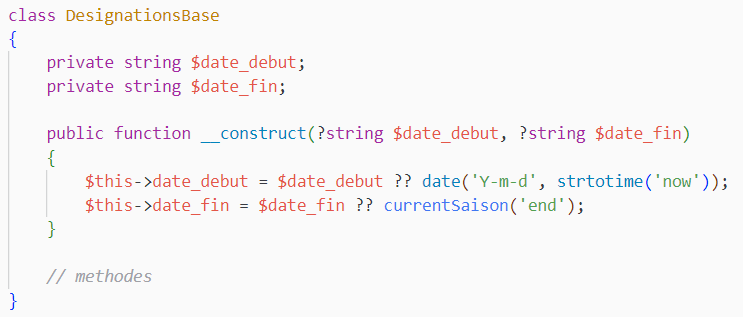
\includegraphics[width=0.75\linewidth]{designations1}
    \caption{Constructeur du composant principal}
\end{figure}

\vspace{1cm}

Ce composant sous forme de classe possède la méthode \colored{group()} qui permet de regrouper les matchs de la période par date, tout en faisant le tri entre les matchs tournois et uniques. 
Cette méthode récupère la liste des dates distinctes de cette période puis associe, pour chaque date, la liste des matchs tournois et uniques à leur tableau des matchs respectifs.

\newpage 

\begin{figure}[!h]
    \centering
    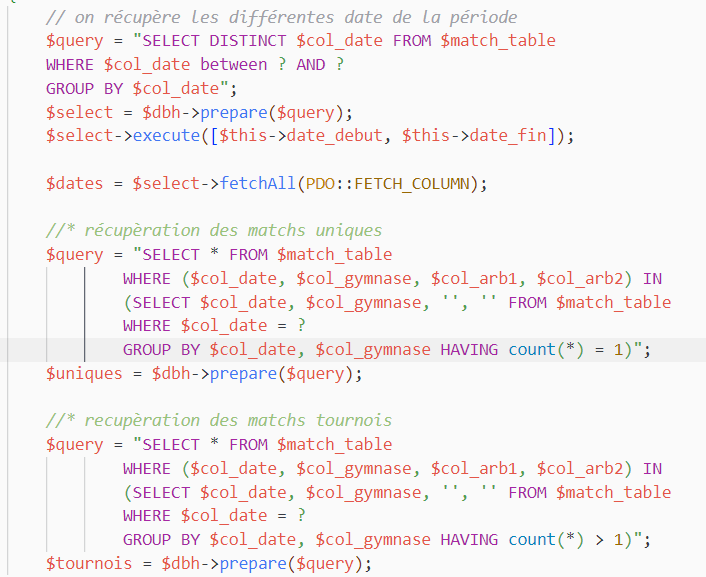
\includegraphics[width=0.75\linewidth]{group1}
    \caption{Préparation des requêtes qui permettent de grouper les matchs}
\end{figure}

\subsection{Etape 2 : récupération des arbitres potentiels}
\vspace{1cm}

Cette liste de dates associées à leurs matchs m’a ensuite permis d’appliquer le premier critère de disponibilité. Pour vérifier les disponibilités des arbitres de chaque match, j’ai réutilisé des méthodes implémentées lors de l’insertion des indisponibilités et des désignations dans la base de données. Alliées ensemble, ces méthode permettent de définir si un arbitre est disponible pour une date donnée. 
Elles m’ont donc permis d’attacher à chaque match un tableau des arbitres disponibles.\\

Ensuite, il a fallut définir pour chaque match une sous liste d’arbitres potentiels habilités à partir de ces tableaux d’arbitres disponibles. 
Pour faire cela j’ai utilisé la classe dédiée au filtre des habilitations en appliquant pour chaque arbitre potentiels une méthode qui renvoi un booléen si l’arbitre est habilité ou non pour le match voulu.